\setchapterstyle{kao}
\setchapterpreamble[u]{\margintoc}
\chapter{Measuring heat and energy flow}
\labch{heat_cool}

\section{Background: Conservation and diffusion (conduction) of heat}
\label{sec:diffusion}

As you probably know from any physics courses you’ve taken, thermal energy can be transferred by radiation, conduction, and, in a liquid or gas, convection (that is, by movement of the fluid). In addition, heat energy is used to change the phase of matter, so the formation/melting of ice and the evaporation/condensation of water vapor are also incredibly important mechanisms for moving heat around. The movement of water vapor from the point where evaporation occurs to the point where precipitation finally releases this energy back to the surrounding atmosphere is a particularly important mechanism for moving heat around the planet. Heat movement through this mechanism is referred to as \emph{latent heat} transfer.

Perhaps the simplest form of heat transfer is heat transfer by conduction. When you touch a solid object with your hand and notice that it feels cool (or warm) to the touch, the primary reason is that heat is being transfer out of (or into) your hand through conduction.  

The basic 1-D equation for conductive heat transfer is a simple differential equation:

\begin{equation} \label{eq:conduction} 
Q =-kA\frac{dT}{dx}
\end{equation}

where $Q$ is the horizontal flow of heat energy (SI units of Joules per second, or Watts, in the x direction), $k$ is a proportionality constant called the thermal conductivity (SI units of Watts per meter per \textdegree C), $A$ is the area through which the energy flows by conduction (SI units m², assumed constant here for simplicity), $T$ is temperature (\textdegree C or K), and $x$ is a horizontal coordinate.  The negative sign is needed ensure that heat is flowing from high temperature to low.  We often write this in terms of a heat flux $q=Q/A$:

\begin{equation} \label{eq:heatflux} 
q =-k\frac{dT}{dx}
\end{equation}

which says that the heat flux (energy flow rate per unit area) is proportional to the temperature gradient $dT/dx$.  The thermal conductivity coefficient $k$ is just the proportionality constant in this relationship.

If the temperature gradient $dT/dx$ is not constant everywhere, there will be more heat flow in some places than others, meaning that there is net movement of thermal energy and thus a change in temperature over time in places where heat inflow does not equal heat outflow.  For a small segment of the system with length $\Delta x$, the change of overall heat energy $\Delta H$ (Joules), is equal to the net difference of heat inflow rate and heat outflow rate, times the time interval over which the accumulation of heat occurs, $\Delta t$:
$\Delta$ (heat energy in segment of length $\Delta x$) =[-(heat outflow at $x+\Delta x$)+(heat inflow at $x$)]$\Delta t$, or

\begin{equation} \label{eq:deltah} 
\Delta H =\left[-\left(-kA \frac{dT}{dx}\bigg\rvert_{(x+\Delta x)}\right)+\left( -kA \frac{dT}{dx}\bigg\rvert_{x}\right)\right]\Delta t
\end{equation}

Now, using the idea that heat content is proportional to temperature: 

\begin{equation} \label{eq:heattransfer} 
\Delta H =cm\Delta T
\end{equation}

where $c$ is the specific heat of the object (Joules/kg/K) and m is its mass (kg).  If the segment we are concerned with has a constant cross-sectional area and a length $\Delta x$, its mass is 
	
\begin{equation} \label{eq:mass} 
\Delta m=\rho V = \rho A \Delta x
\end{equation}

where $\rho$ is the density of the object (kg/m³).

With a few substitutions, it is simple to show that 	

\begin{equation} \label{eq:deltaH2} 
\Delta H =c\rho A\Delta x \Delta T
\end{equation}


Substituting into \refeq{deltah} and dividing by $c \rho A \Delta x \Delta t$:

\begin{equation} \label{eq:tempgradient} 
\frac{\Delta T}{\Delta t} =\frac{k}{\rho c}\frac{\left. \frac{dT}{dx}\right|_{x+\Delta x}-\left. \frac{dT}{dx}\right|_{x}}{\Delta x}
\end{equation}

Taking the limit as $\Delta x \rightarrow 0 $:

\begin{equation} \label{eq:secondderivative} 
\frac{\Delta T}{\Delta t}=\frac{k}{\rho c}\frac{d}{dx}\left ( \frac{dT}{dx} \right )=\frac{k}{\rho c}\frac{d^{2}T}{dx^2}
\end{equation}

If we also take the limit as $\Delta t \rightarrow 0$, this results in something referred to as a partial differential equation (it is customary to use the symbol $\partial$ to represent the gradient instead of $d$ when the gradient can be computed in two different directions—here $x$ and $t$--but the meaning is the same):

\begin{equation} \label{eq:diffusion1} 
\frac{\partial T}{\partial t}=\frac{k}{\rho c}\frac{d^{2}T}{dx^2} 
\end{equation}

Seeing as how $k$, $\rho$ and $c$ are all properties of the material that is doing the conducting, it is customary to lump them all into a single coefficient we’ll call $\kappa$, usually referred to as a diffusion coefficient (units of m²/t).  

\begin{equation} \label{eq:diffusion} 
\frac{\partial T}{\partial t}=\kappa \frac{\partial ^{2}T}{\partial x^2} 
\end{equation}

\refeq{diffusion} is called the diffusion equation and is very well known.  It says that the time rate of change of temperature is proportional to the spatial gradient of the spatial gradient of temperature (in other words, to the spatial curvature of temperature).  In places where there is high curvature, temperature changes quickly.  However, given enough time, all the imbalances should diffuse away, leaving behind a linear temperature profile with constant slope that experiences no change in temperature over time.  This is illustrated in \reffig{diffusionplot}, which is a numerical solution to the equation (with a diffusivity coefficient for iron), starting with the system at 50 \textdegree C everywhere and then with each end of the bar instantaneously heated/cooled to 100\textdegree C or 0 \textdegree C, respectively.  

\begin{marginfigure}[-3cm]
	\begin{center}
		\includegraphics[height=7cm]{Images/diffusionplot.png}
		\caption[Numerical Solution to Diffusion Equation]{Simulated temperature profiles for a one-meter long iron bar.  The bar is initially held at 50 \textdegree C at time zero, when one end is placed in a 100 \textdegree C bath and the other in a 0 \textdegree C bath.  .}
		\labfig{diffusionplot}
	\end{center}
\end{marginfigure}

\section{\color{gray} Evaporative cooling \color{black}}
\section{Heat transfer by conduction}

This experiment is intended to measure the types of profiles that were discussed in the background to this chapter.  To accomplish this, we will use a one meter long rod as the metal through which heat is conducted. The experimental setup is illustrated in \reffig{hotcold}.  We will start with the metal at room temperature and then place one end in a large bath of warm water and the other end in a separate bath of ice water (the rod will be bent in order to accomplish this).  We will set up five temperature probes on each bar at regular intervals, tape them (carefully) to the bar (\reffig{bar_sensors_cropped}) and then cover them with an insulating pipe wrap (\reffig{insulated_bar}) to ensure that heat is not transferred to/from the atmosphere during the experiment.

\begin{marginfigure}[-5cm]
	\begin{center}
		\includegraphics[height=7cm]{Images/diffusion_experiment.png}
		\caption[Diffusion Experiment]{Basic setup for heat transfer by conduction experiment.}
		\labfig{hotcold}
	\end{center}
\end{marginfigure}

\begin{marginfigure}[3cm]
	\begin{center}
		\includegraphics[height=7cm]{Images/bar_sensors_cropped.jpg}
		\caption[Sensors on Metal Rod]{Sensors are taped to the metal rod to ensure that conduction between sensor and rod is good. This helps ensure that the temperature sensor has a similar temperature to the rod it is in contact with.}
		\labfig{bar_sensors_cropped}
	\end{center}
\end{marginfigure}


Hook up the probes as instructed in \refch{digital_interfaces}, with all probes connected individually (i.e., in parallel) to the 3.3V pin on the microcontroller board (red wire), ground (black wire) and a \texttt{GPIO} pin (yellow wire). The SDA pin (\texttt{GPIO} 3 on the Adafruit Feather ESP32-S2) is often a good choice because it often includes a pull-up resistor. You will need to use a breadboard or solder to make the connections.  Remember to include a roughly 4.7 kOhm resistor between the data and power pins if you are not using a pin with an internal pull-up resistor.
 
Note that it may be easier to manage the many wires if you simply solder all wires of a given color together, as illustrated in \reffig{fiveDS18B20series}, ensuring a good connection and simplifying layout significantly.

Use the code snippets presented in \refch{digital_interfaces} to write a program that can read temperature data from five separate probes. As suggested in the milestone for the \texttt{DS18B20}, you may need to do some testing to determine which sensor is which (i.e., which identifier in the “roms” variable corresponds with which probe).  It is probably easiest to do this by hooking up all the sensors and printing the results to the screen once every few seconds.  Then warm a given sensor in your hand to identify the position of this sensor in the output text string (i.e., first, second, … , fifth).  Write this number on a piece of tape that you attach to the sensor. It is helpful to then hook the sensors up to the bar in the order that the variable “roms” records them. Your notes should be sufficiently clear so that someone reviewing your work understands and can repeat what you do.

You may then use the data logging program listed below to save your data. The program prints the results from each sensor to the screen as well as to a file on the device.  It  adds a timestamp to a data log file each time the program is run, so if your program is interrupted in the middle of the experiment, you will be able to restart and should be able to determine where you are in the run. (Note that your microcontroller can only keep track of time if it does not lose power.  However, if you are using Thonny as your development environment, it will reset the microcontrollers real time clock when you start.)  Make any necessary modifications so that the program logs data at a resonable time interval.

\begin{marginfigure}[]
	\begin{center}
		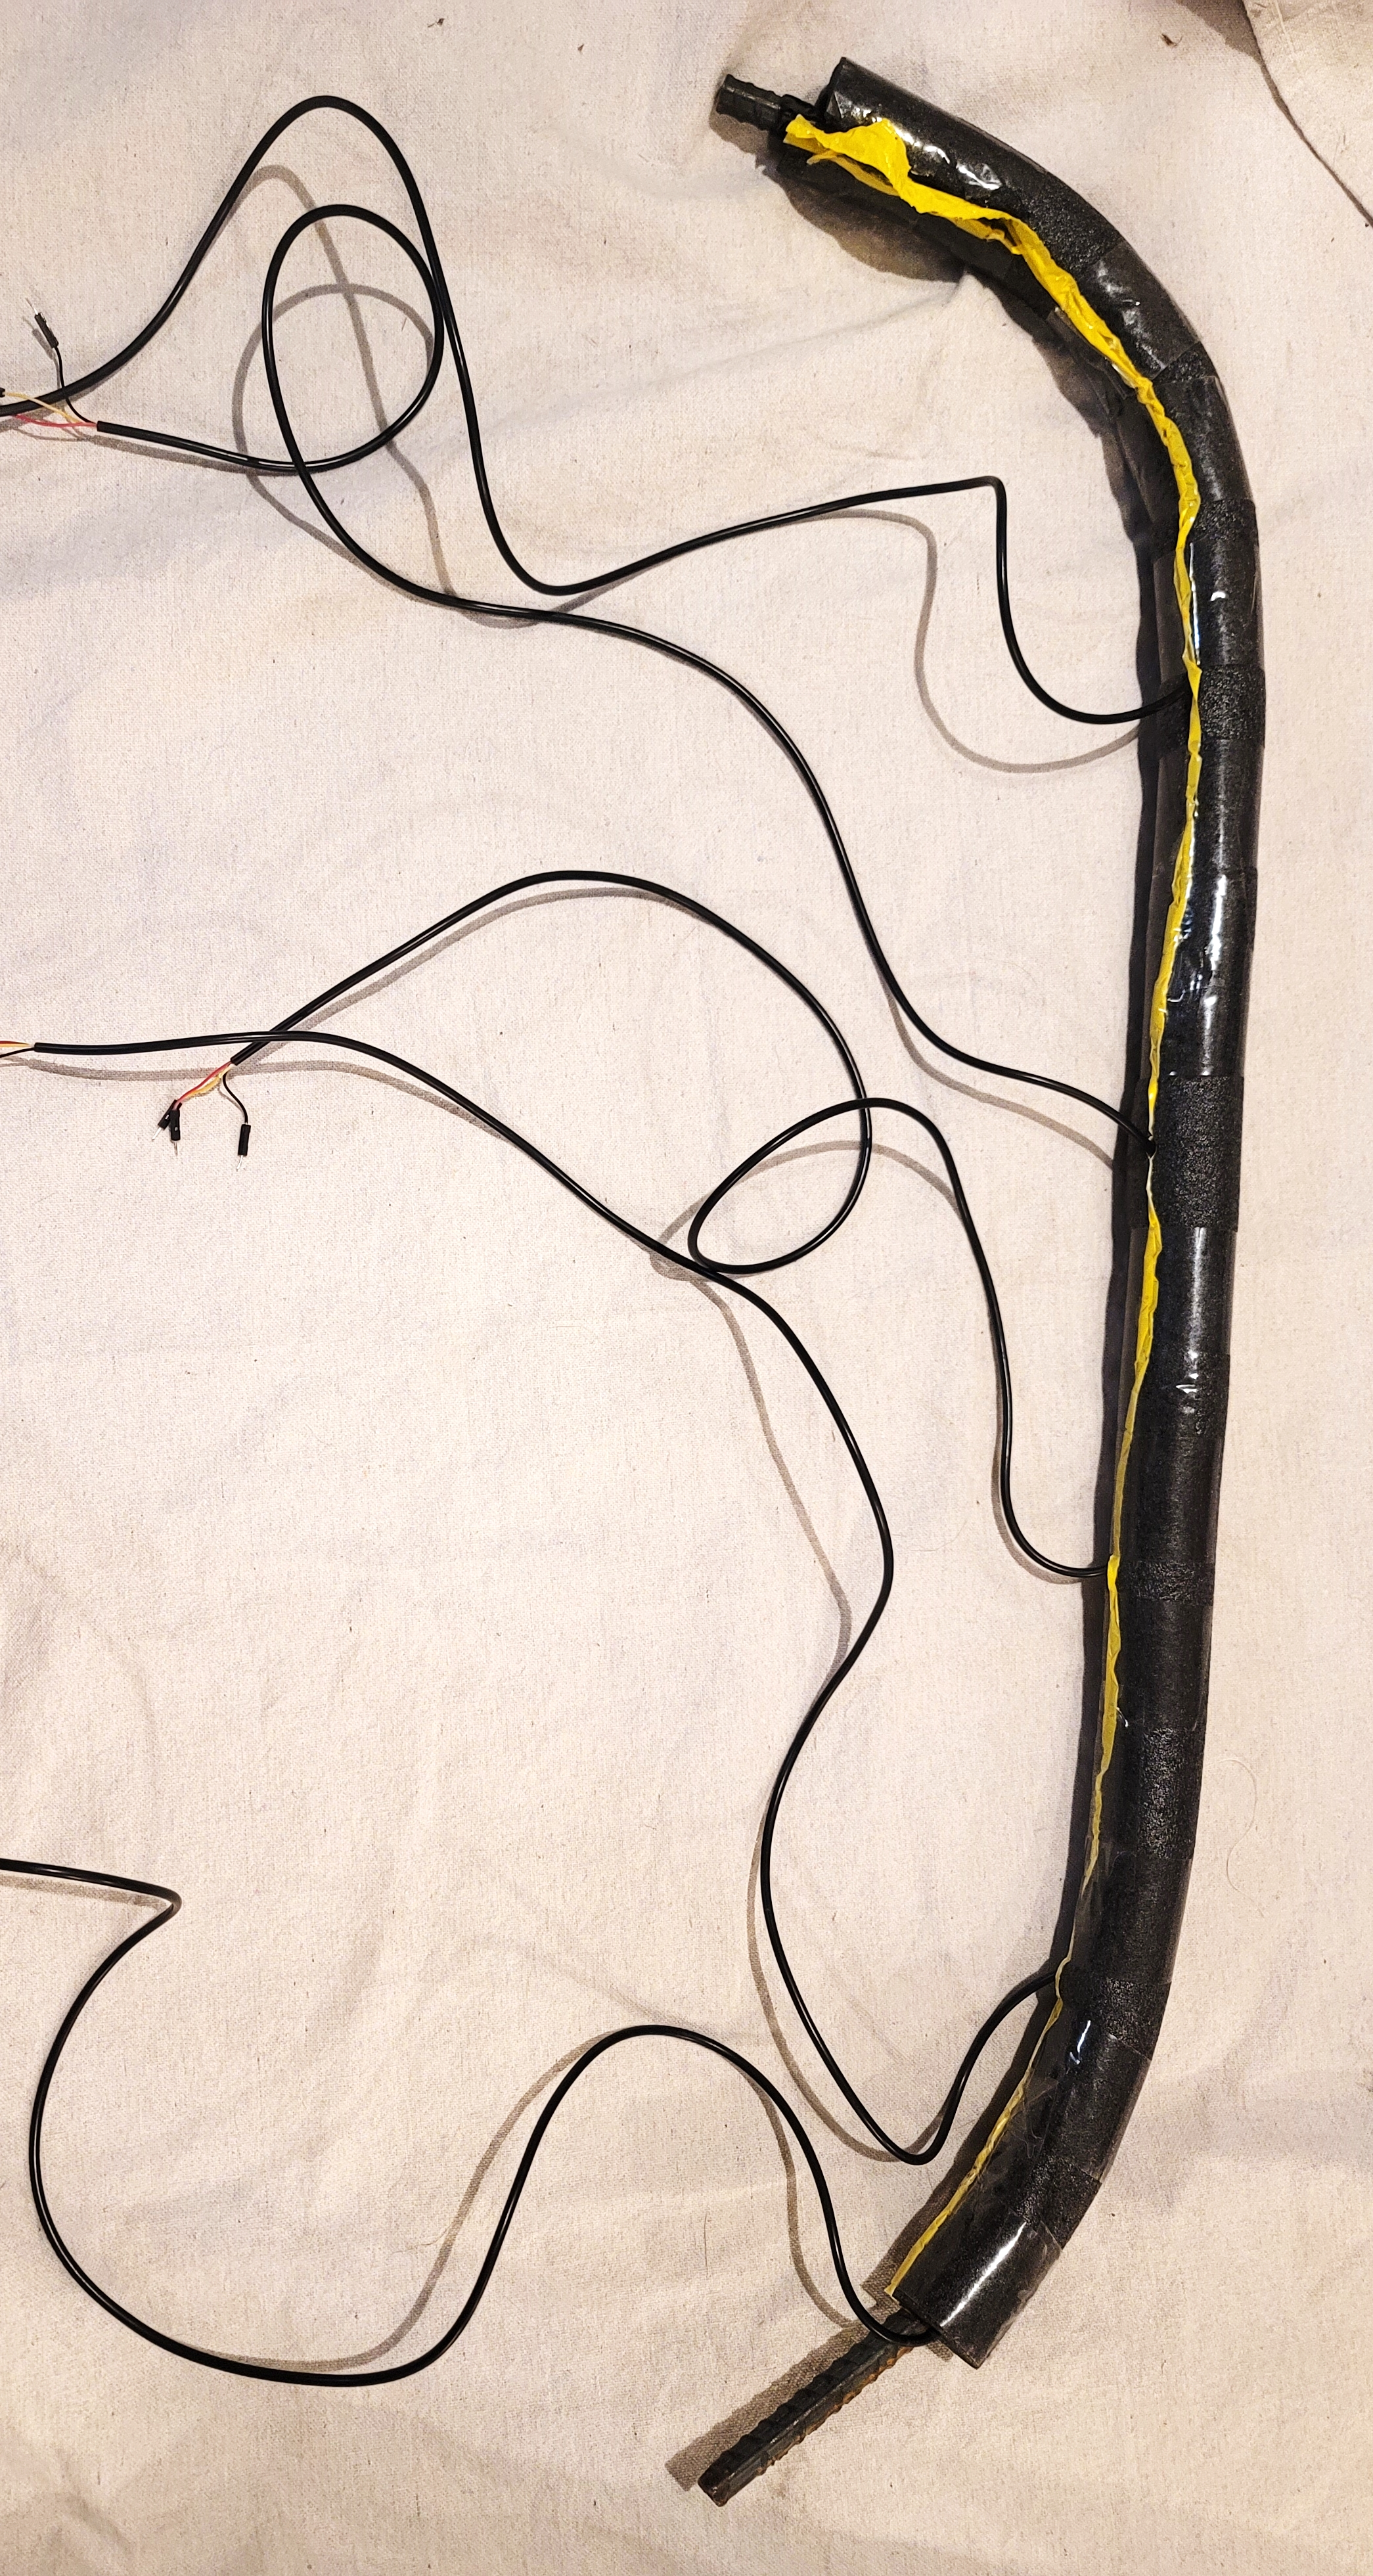
\includegraphics[height=7cm]{Images/insulated_bar.jpg}
		\caption[Insulated Bar for Diffusion Experiment]{\texttt{DS18B20} sensors on rod covered with pipe insulation.}
		\labfig{insulated_bar}
	\end{center}
\end{marginfigure}

Once you confirm that the data logging program is working and is loggin at an appropriate interval, you may begin the experiment by placing the two ends of your metal rod into the warm- and cold-water baths.  Be sure to record the time when you do this, particularly if you are already running the datalogging program. If you are using Thonny for your REPL, you may track the progress of the experiment by enabling the plotter window under the ``View'' menu. As you watch the temperatures change over the course of the experiment, think about how you will know when the system reaches a steady state.

Once data collection is complete, stop your program from running by pressing “Control C” or the “Stop” button. Then copy your “datalog.txt” file from the microcontroller to the computer using the file management utilities on Thonny, mpfShell, or WebREPL. You should view the file and clean up any extraneous data that do not correspond to experimental data (e.g., any data in the file that remains from the time you were testing to confirm that the equipment was working).

\subsection{Code for use in conduction experiment}

\begin{lstlisting}[language=Python]
#import all required libraries
import machine 
import time  
import onewire, ds18x20
import os
from machine import Pin

#define addresses of each sensor
dat = machine.Pin(3)  #SDA on Adafruit Feather ESP32-S2
ds = ds18x20.DS18X20(onewire.OneWire(dat))
roms = ds.scan()
print("found devices:", roms)

#format time
t = time.localtime()
started = f"starting at {t[0]}-{t[1]}-{t[2]} {t[3]}:{t[4]}:{t[5]}"

#format write string for header
text = started + ("\r\n")
text = text + "minutes"
for i in range(len(roms)):
    text = text + f",temperature{i}"
print(text)
text_to_write = text + ("\r\n")

#Write the header line
#uncomment next line to erase the file each time you start
#f=open("datalog.txt","w")  #opening as write clears all data
f=open("datalog.txt","a")  #opening as append does not clear data
f.write(text_to_write)
f.close()

#set up timing
dt = 3
initial_time = time.time()
next_time = initial_time

while True:    
    if time.time()>=next_time:
        next_time = next_time + dt
        time_in_run = time.time() - initial_time
        
        ds.convert_temp()
        time.sleep_ms(750)   #wait long enough for sensors to respond
        
        #format the write string for data line
        text = (f"{time_in_run/60}")
        for rom in roms:
            temperature = ds.read_temp(rom)
            text = text + (f",{temperature:.1f}") 
        print(text)
        text_to_write = text+("\r\n")
        
        #write to file
        f=open("datalog.txt","a")
        f.write(text_to_write)
        f.close()
    else:
        time.sleep(0.1)
\end{lstlisting}

\newpage

\subsection{Numerical solution to diffusion equation and comparison with student data}

In section \ref{sec:diffusion}, we presented a derivation of the diffusion equation, the equation that governs the flow of heat through a solid object. The equation is repeated here for clarity.

\begin{equation} \label{eq:diffusion_again} 
\frac{\partial T}{\partial t}=\kappa \frac{\partial ^{2}T}{\partial x^2} 
\end{equation}

The details of the various possible numerical solutions to this equation are beyond the scope of this textbook.  However, the essence can be understood by recognizing that any derivative can be written as a slope of dependent variable (e.g., of temperature T) in the direction of the independent variable of interest, t or x.

\begin{equation} \label{eq:dTdt} 
\frac{\partial T\left ( x,t \right )}{\partial t}\approx  \frac{\Delta T}{\Delta t}\approx \frac{T\left ( x,t+\Delta t \right )-T\left ( x,t \right )}{\Delta t}
\end{equation}

\begin{equation} \label{eq:dTdx} 
\frac{\partial T\left ( x,t \right )}{\partial x}\approx  \frac{\Delta T}{\Delta x}\approx \frac{T\left ( x+\Delta x,t \right )-T\left ( x,t \right )}{\Delta x}
\end{equation}

You might notice that the approximations in \ref{eq:dTdt} and \ref{eq:dTdx} are quite similar to the basic assumptions in \ref{sec:diffusion} that allowed us to derive the differential equation in the first place.

We can also discretize a second-order derivative by considering a point half-way between $x\!-\!\Delta \!x$ and ${x}$ and then another point half-way between $x$ and  $x\!+\!\Delta \!x$. These two points are a distance $\frac{1}{2}\Delta x +\frac{1}{2}\Delta x=\Delta x $ apart. If we approximate the first derivative at each of these points using an equation of the form of \ref{eq:dTdx}, we can then approximate the second-order spatial derivative $d^2T/dx^2$ as follows.

\begin{equation} \label{eq:centered} 
\begin{split}
\frac{\partial^2 T}{\partial x^2}&= \frac{\partial }{\partial x}\left ( \frac{\partial T\left ( x,t \right )}{\partial x} \right )\approx \frac {\Delta\left ( \frac{\Delta T}{\Delta x} \right )}{\Delta x}
\\
&\approx \frac{\left [ \frac{T\left ( x+\Delta x,t \right )-T\left ( x,t \right )}{\Delta x} \right ]-\left [ \frac{T\left ( x,t \right )-T\left ( x-\Delta x,t \right )}{\Delta x} \right ]}{\Delta x}
\end{split}
\end{equation}

With a little algebra, this simplifies to 

\begin{equation} \label{eq:centered} 
\frac{\partial^2 T}{\partial x^2}\approx \frac{T\left ( x+\Delta x,t \right )-2T\left ( x,t \right )+T\left ( x-\Delta x,t \right )}{\Delta x^{2}}
\end{equation}

Substituting equations \ref{eq:dTdt} and \ref{eq:centered} into equation \ref{eq:diffusion_again} and doing some more algebra yields

\begin{equation} \label{eq:FTCS} 
T\!\left ( x,t\!+\!\Delta t \right ) \approx T\!\left ( x,t \right )+\frac{\kappa \Delta t}{\Delta x^{2}}\left ( T\!\left ( x\!+\!\Delta x\!,\!t \right ) -2T\!\left ( x,t \right )+T\!\left ( x\!-\!\Delta x,t \right )\right )
\end{equation}

Equation \ref{eq:FTCS} what is known as a finite difference solution to the differential equation. This particular form, where we assumed spatial derivatives were centered around the point of interest, is known as the forward in time/centered in space approximation. There are other approximations that allow for longer steps of time $\Delta t$ without leading to numerical instability, but in essentially all cases, these solutions can be used to solve for temperature $T$ at any timestep in the simulation as long as an initial temperature is known everywhere in the system at the beginning of the simulation (the \emph{initial condition}), and as long as temperature is known at the edge of the system during the entire simulation (the \emph{boundary condition}.  For the experiment with the metal rod, the initial condition represents the rod's temperature before the experiment begins, and the boundary conditions are the temperatures in the two water baths on either end of the rod.  

\begin{table}[h]
\caption[1.1.1. materials]{\textbf{Heat transfer properties for selected materials.}}	
\label{tab:conductivity_properties}	
	\renewcommand{\arraystretch}{1.5}
	\begin{NiceTabular}{@{}m{2.0cm}| m{1.2cm} |m{1cm}| m{.8cm} m{.8cm} m{.75cm} m{.7cm} m{.8cm}@{}}
		\CodeBefore
		\Body
		\hline
			
		Variable &\hfil Symbol &\hfil Units& Cop-per&Alu-minum&Wood&Con-crete&Steel \\
		\hline
		Thermal conductivity\tabularnote{\footnotesize{from \htmladdnormallink{https://www.engineeringtoolbox.com/thermal-conductivity-d\textunderscore429.html}{https://www.engineeringtoolbox.com/thermal-conductivity-d_429.html}}} & \hfil $k$  &\hfil $\frac{J}{msK}$& 401&205&0.12&0.85&43 \\
		Specific heat\tabularnote{\footnotesize{from \htmladdnormallink{https://www.engineeringtoolbox.com/specific-heat-capacity-d\_391.html}{https://www.engineeringtoolbox.com/specific-heat-capacity-d_391.html}}} &\hfil $c$ & \hfil $\frac{J}{kg K}$ &385 & 897&1300-2400&880&490 \\
		Density\tabularnote{\footnotesize{from \htmladdnormallink{https://www.engineeringtoolbox.com/density-solids-d\_1265.html}{https://www.engineeringtoolbox.com/density-solids-d_1265.html}}} &\hfil $\rho$ &\hfil $\frac{kg}{m^3}$ &8790 & 2700&530&1500&7890 \\
		Diffusion coefficient & \hfil $\kappa$&\hfil $\frac{m^2}{s}$&\num{1.18e-4}&\num{8.55E-05}&\num{1.51e-06}&\num{7.56E-07}&\num{1.11E-05}\\

		\hline
	\end{NiceTabular}
\end{table}

The solution requires several input parameters associated with material properties. Values for selected materials are presented in Table \ref{tab:conductivity_properties}. In the table, values for the diffusion coefficient have been computed from the material properties according to the definition for $\kappa$ we used in Section \ref{sec:diffusion}.

\begin{equation} \label{eq:diffusion_coef} 
\kappa=\frac{k}{\rho c}
\end{equation}

\subsection{Code for implementing numerical solution to diffusion equation}

It is straightforward to define an algorithm to solve Equation \ref{eq:diffusion_again} by stepping forward in time using Equation \ref{eq:FTCS}. To accomplish this in Python, we first import the numpy library, then define all the parameters we want to use for the solution.

\begin{lstlisting}[language=Python]
import numpy as np

dx = 0.05    #length of spatial step
L = 1        #length of bar in meters
dt = 10       #seconds
tmax = 4000   #seconds
k = 100        #J/s/m/K
c = 900      #J/kg/K
rho = 2700   #density, kg/m3
kappa = k/(c*rho) #diffusion coef
\end{lstlisting}

Then define the initial and boundary conditions.

\begin{lstlisting}[language=Python]
T0 = 50      #initial condition, degrees C
Tleft = 100    #left boundary, degrees C
Tright = 0 #right boundary, degrees C
\end{lstlisting}

Once those are set, we can set up a grid of points (so all x- and t- values) at which we wish to compute temperature $T$.  Here, the values of x at which computations occur are computed using the spatial step $dx$ that we set previously. We also determine the times when we will perform the computation using the $dt$ we set previously.

\begin{lstlisting}[language=Python]
x = np.arange(0,L+dx,dx)
t = np.arange(0,tmax+dt,dt)
\end{lstlisting}

We can think of our solution domain as a table of points, with columns representing x-values and rows representing t-values. In order to apply this, we need to know the number of x-values and t-values we'll need.  These can be found, respectively, by dividing our bar length by the spatial step dx or by dividing the simulated time period we wish to simulate by the time step dt.

\begin{lstlisting}[language=Python]
columnmax = int(L/dx)
rowmax = int(tmax/dt)
\end{lstlisting}

We now create a blank table of points (technically a 2-D numpy array) of blank temperature values. Here, we'll set up the array using a function in numpy that creates an array and assigns the value `one' to each value. We then reset the values of the first row and the first and last columns to the initial and boundary temperatures we defined previously, as appropriate.

\begin{lstlisting}[language=Python]
T=np.ones((rowmax+1,columnmax+1))
T[0,...]=T0
T[...,0] = Tleft
T[...,columnmax] = Tright
\end{lstlisting}

All we need to do now is to implement the recursive equation to fill in the temperature values for all the non-boundary cells in the array.  We accomplish this here using a set of nested loops.  The first (outer) loop goes through every row (aka every time for which a solution is desired).  Then for each row, we compute the value in each column by looping through the columns and implementing Equation \ref{eq:FTCS}.

\begin{lstlisting}[language=Python]
#start at row 0 and go to the last row
for i in range(0,rowmax):   
    #start at column 1 and go to the last column
    for m in range(1,columnmax):  
        T[i+1,m]=T[i,m]+ kappa * dt/dx**2*(T[i,m+1]-2*T[i,m]+T[i,m-1])
\end{lstlisting}

That's it--we just computed a temperature for every point in our large array! The basic numerical results can be displayed in the REPL with a simple `print' statment.
\begin{lstlisting}[language=Python]
print(T)
\end{lstlisting}

Note that if the timestep $dt$ is too long or if the spatial step $dx$ is too short, the solution can become unstable. If results appear to oscillate in an unreasonable way, or worse, if the program crashes, try increasing the spatial step and/or decreasing the time step, then re-running.

All that's left is to visualize the results. While we provided a graph illustrating the solution  in \reffig{diffusionplot}, the procedures for creating these graphs are left as an exercise for students. The interactive \htmladdnormallink{Jupyter notebook on the diffusion equation}{https://github.com/jwlauer/EnvironmentalSensing/blob/master/AnalysisCode/DiffusionAnimation/DiffusionAndAnimation.ipynb} provides step-by-step guidance, including detailed instructions for creating an animation that illustrates the evolution of the numerical results over time.

\loadMilestone{mlst:08a} % load milestone with tags id: mlst:05e 
\newpage

\section{\color{gray} Heating and cooling of lakes and oceans \color{black}}
\section{\color{gray} Thermoelectric (Peltier) heating and cooling \color{black}}